\documentclass{article}
\usepackage{tikz}
\usetikzlibrary{arrows.meta}

\begin{document}

\begin{figure}[h]
    \centering
    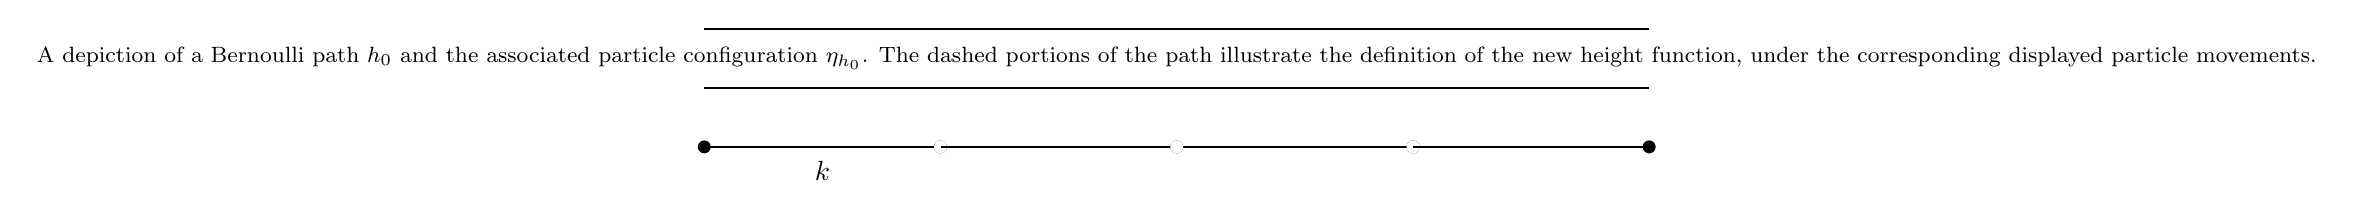
\begin{tikzpicture}[scale=1.5]
        % Draw the path h_0
        \draw[thick] (0,0) -- (2,0);
        \draw[thick] (2,0) -- (4,0);
        \draw[thick] (4,0) -- (6,0);
        \draw[thick] (6,0) -- (8,0);
        
        % Draw the dashed path
        \draw[dashed, thick] (0,0.5) -- (2,0.5);
        \draw[dashed, thick] (2,0.5) -- (4,0.5);
        \draw[dashed, thick] (4,0.5) -- (6,0.5);
        \draw[dashed, thick] (6,0.5) -- (8,0.5);
        
        % Draw the horizontal line at y=0.5
        \draw[thick] (0,0.5) -- (8,0.5);
        
        % Draw the horizontal line at y=0
        \draw[thick] (0,-0.5) -- (8,-0.5);
        
        % Draw the circles representing particles
        \foreach \x in {0,2,...,8} {
            \filldraw[black] (\x,-0.5) circle (0.05);
        }
        \foreach \x in {2,4,6} {
            \filldraw[white] (\x,-0.5) circle (0.05);
        }
        
        % Draw the labels for the circles
        \node at (1,-0.7) {$k$};
        
        % Draw the dashed lines connecting the circles
        \draw[dashed, thick] (2,-0.5) to[out=0,in=180] (3,-0.5);
        \draw[dashed, thick] (6,-0.5) to[out=0,in=180] (7,-0.5);
        
        % Caption
        \node at (4,0.25) {\footnotesize A depiction of a Bernoulli path $h_0$ and the associated particle configuration $\eta_{h_0}$. The dashed portions of the path illustrate the definition of the new height function, under the corresponding displayed particle movements.};
    \end{tikzpicture}
\end{figure}

\end{document}